%@@@@@@@@@@@@@@@@@@@@@@@@@@@@@@@@@@@@@@@@@@@@@@@@@@@@@@@@@@@@@@@@@@@@@@@
\chapter{Components} \label{c:components}
%@@@@@@@@@@@@@@@@@@@@@@@@@@@@@@@@@@@@@@@@@@@@@@@@@@@@@@@@@@@@@@@@@@@@@@@

% \centerline{\includegraphics{uml/core-components.1}}


\centerline{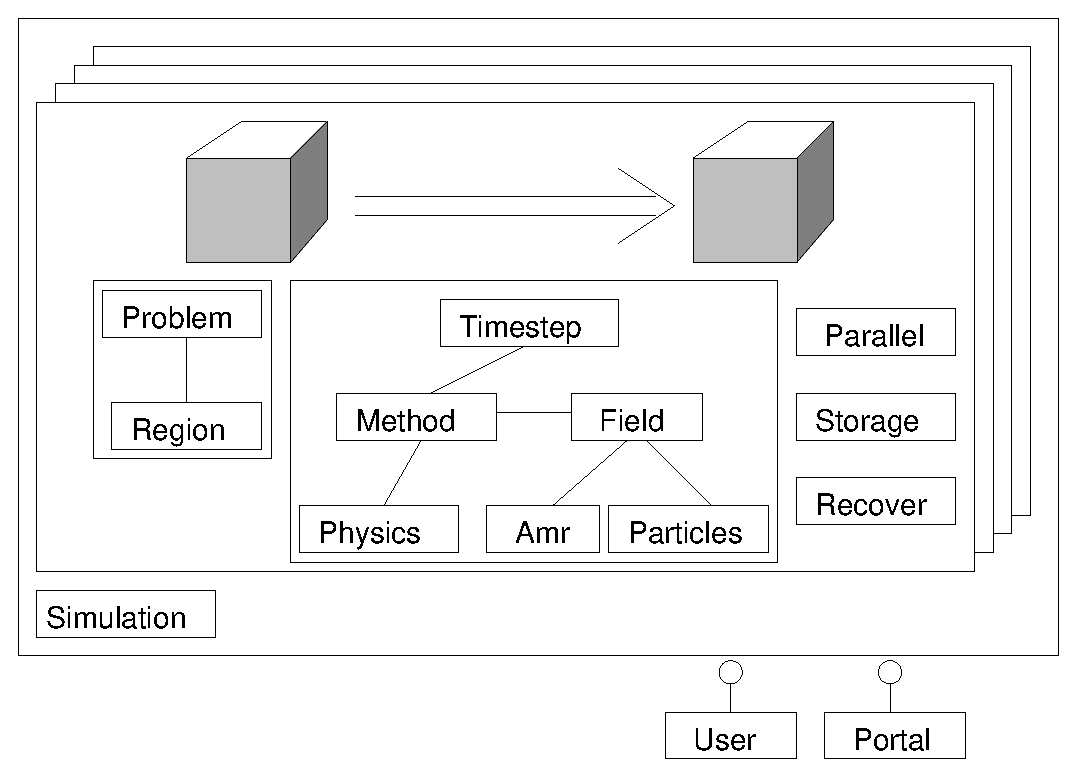
\includegraphics[totalheight=3in]{components.eps}}

   This chapter describes the design of \cello\ at the component
   level.  Each component is described, including the component
   interdependencies, interface, and classes.

\begin{description}
%
 \item [\todo Mesh (\S\ref{s:component-amr}): ]
%
        The \code{Mesh} component includes classes for representing
        multi-resolution data on a hierarchy of grid patches of
        varying spacial resolutions.  The \code{Mesh} data
        structures can have multiple levels of data distribution and
        parallelism.  Uses the \code{Parallel} component for
        controlling the parallel communication, synchronization, and
        load-balancing.
%
 \item [\todo Array (\S\ref{s:component-array}): ]
%
        The \code{Array} component is used for representing a single
        array of up to $3$ dimensions.  The \code{Array} may include
        options for MPI-, OMP-, UPC-, or GPU-based parallelism, as
        well as options for controlling memory layout to improve cache
        performance.
%
 \item [\todo Disk (\S\ref{s:component-disk}): ]
%
        The \code{Disk} component controls what, when, and how to
        input and output large-scale data to long-term permanent
        storage, primarily \code{Fields} (represented as
        \code{Particles} or \code{Arrays}).
%
 \item [\todo Error (\S\ref{s:component-error}): ]
%
        The \code{Error} package is used to detect errors, evaluate
        them, and decide what to do about them.  This includes
        maintaining restart data dumps, and may involve shutting down
        a processor or node and rebalancing the data, etc.
%
 \item [\todo Field (\S\ref{s:component-field}): ]
%
        A \code{Field} is used to represent a specific continuous
        scalar or vector field.  The actual \code{Field} is
        represented either using adaptive mesh refinement via
        \code{Mesh}, or as a collection of particles using
        \code{Particles}.  Includes \code{Units} to define the problem
        units, as well as scaling amount to improve numerics, and
        scaling quantization to avoid precision loss.
%
 \item [\todo Memory (\S\ref{s:component-memory}): ]
%
        The \code{Memory} component controls dynamic memory
        allocation, and includes features for monitoring memory usage,
        improving performance, and verifying correctness.
%
 \item [\todo Method (\S\ref{s:component-method}): ]
%
        Defines how to simulate the physics in the computational
        universe.  A \code{Method} specifies the numerical method to
        use, which \code{Field}s are involved, and any associated
        method-specific parameters.  Sequencing and coupling of
        \code{Method}s is defined in \code{Problem} and implemented in
        \code{Control}.  Analysis and visualization are considered
        \code{Method}s as well.
%
 \item [\todo Monitor (\S\ref{s:component-monitor}): ]
%
        The \code{Monitor} component controls what and when to output
        user-readable summary information about the running
        application, such as status summary, progress, warnings,
        errors, and performance information.
%
 \item [\todo Parallel (\S\ref{s:component-parallel}): ]
%
        The \code{Parallel} component is used to specify and control
        the levels of parallelizion (simulations, patches, and
        subblocks), type of parallelization (shared- or
        distributed-memory), and mechanism for controling the
        parallelism (MPI-1 2-sided, MPI-2 1-sided, OpenMP, UPC).
        Lower-level parameters provide detailed control of buffering,
        blocking or nonblocking, patch-to-processor mapping,
        subblock-to-thread mapping, etc.
%
 \item [\todo Parameters (\S\ref{s:component-parameters}): ]
%
        The \code{Parameters} component
        reads in a parameter file or files, and provides the
        application access to parameter values.
%
 \item [\todo Particles (\S\ref{s:component-particles}): ]
%
        The \code{Particles} component serves to represent multi-level
        parallel distribution of sets of various types of particle
        data.  Uses the \code{Parallel} component for controlling the
        parallel communication, synchronization, distribution, and
        load-balancing of \code{Particles}.
%
 \item [\todo Performance (\S\ref{s:component-performance}): ]
%
        The \code{Performance} component monitors performance such as
        memory usage, computation amount, parallel communication,
        parallel load balancing, disk storage, etc., and provides
        access functions to be called from other components.
%
 \item [\todo Portal (\S\ref{s:component-portal}): ]
%
        The \code{Portal} component controls the interaction of the
        application with external applications, for both obtaining
        information about a running simulation, and controling it.
%
 \item [\done Problem (\S\ref{s:component-problem}): ]
%
   A \code{Problem} defines and manages an astrophysics problem,
   including defining \code{Physics} parameters, the domain and
   initial conditions, and boundary condition type and values.
%
%
 \item [\done Simulation (\S\ref{s:component-simulation}): ]
%
   A \code{Simulation} defines and manages a computational
   astrophysics \code{Problem} or an ensemble of related
   \code{Problem}s. Invokes \code{Control} to advance the
   \code{Problem}(s), and may call the \code{Parallel} component to
   manage the high-level parallelization of multiple \code{Problem}s
   in an ensemble.
%
 \item [\todo Control (\S\ref{s:component-control}): ]
%
        \code{Control} handles the timestepping of methods to advance
        the problem forward in time.
\end{description}

%-----------------------------------------------------------------------

%=======================================================================
\section{AMR Component} \label{s:component-amr}
%=======================================================================

Specify data structures and data structure parameters for distributed
AMR hierarchies, such as number of mesh levels, grid patch properties,
rebuild algorithm, dynamic load balancing, refinement criteria, etc.

Hierarchy
Array


\begin{itemize}
\item hierarchy
\begin{item}
\item min\_levels 
\item max\_levels 
\end{item}
\item level
\item grid
\begin{itemize}
\item min\_size
\item max\_size
\item max\_aspect
\item quantum
\end{itemize}
\end{itemize}

\centerline{
\includegraphics[width=1.8in]{amr4-1.eps} \ \
            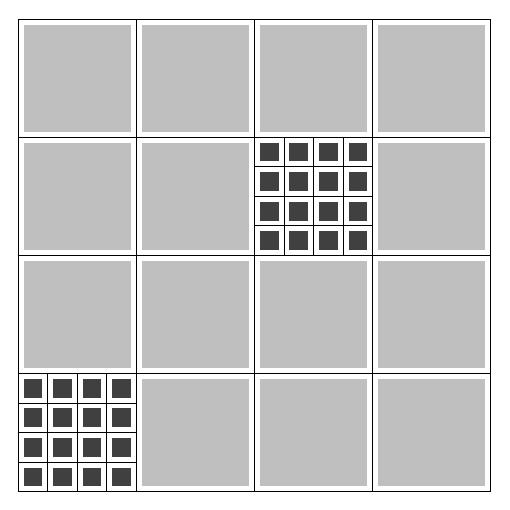
\includegraphics[width=1.8in]{amr4-2.eps} \ \
            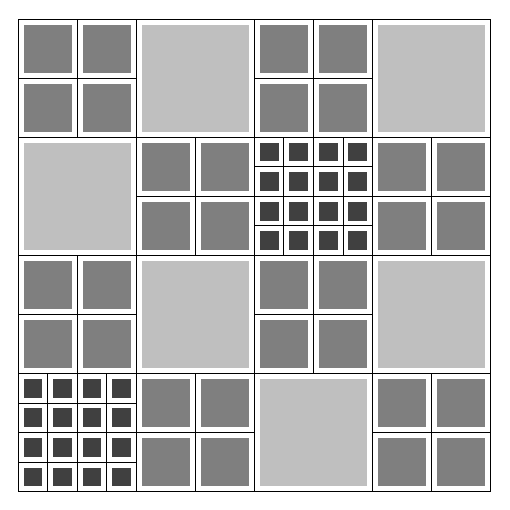
\includegraphics[width=1.8in]{amr4-3.eps}}

\centerline{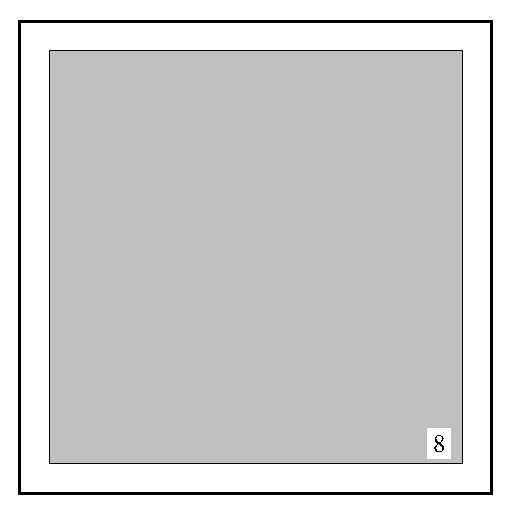
\includegraphics[width=1.8in]{amr2-1.eps} \ \
            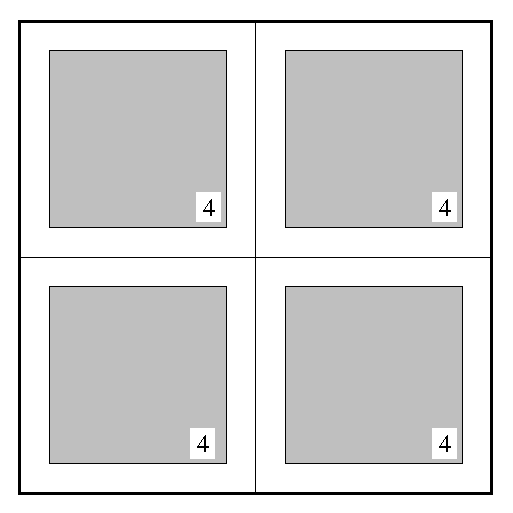
\includegraphics[width=1.8in]{amr2-2.eps} \ \
            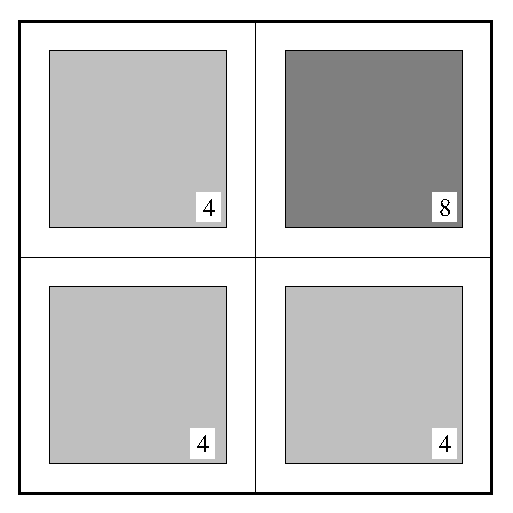
\includegraphics[width=1.8in]{amr2-3.eps}}
\ \\
\centerline{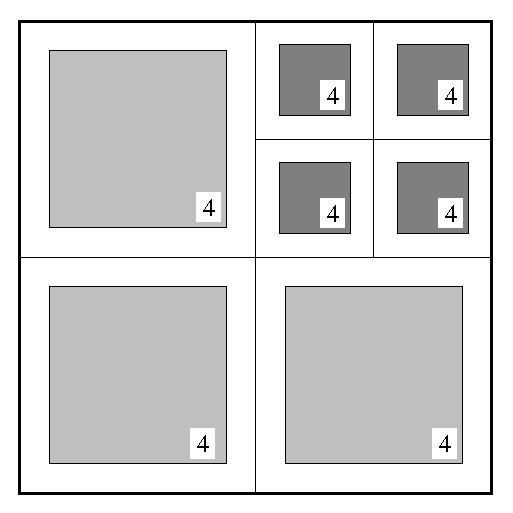
\includegraphics[width=1.8in]{amr2-4.eps} \ \
            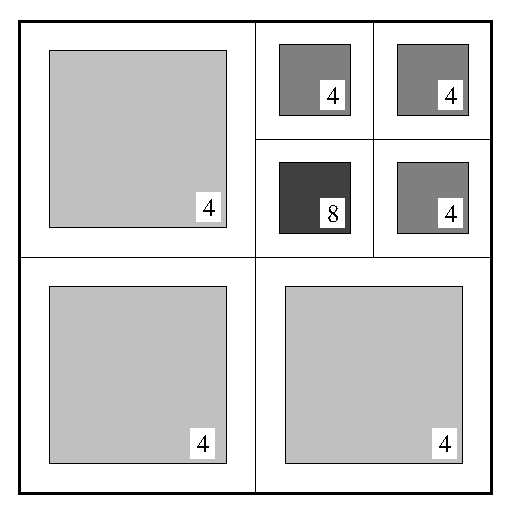
\includegraphics[width=1.8in]{amr2-5.eps} \ \
            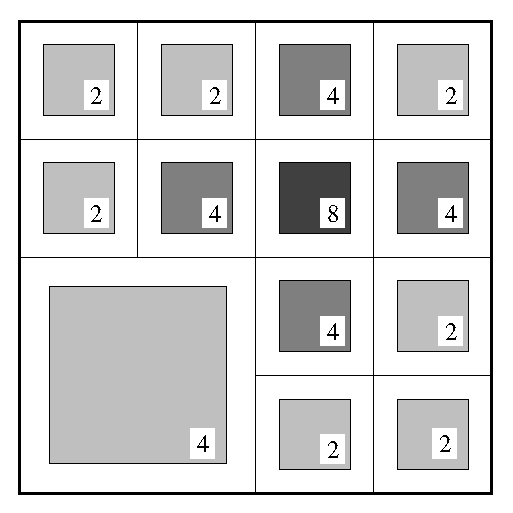
\includegraphics[width=1.8in]{amr2-7.eps}}
\ \\
\centerline{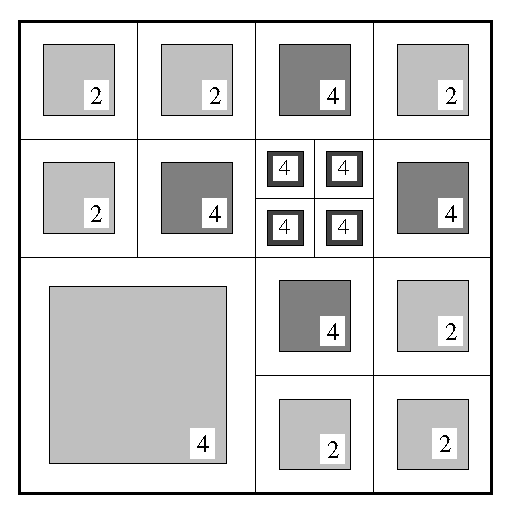
\includegraphics[width=1.8in]{amr2-8.eps} \ \
            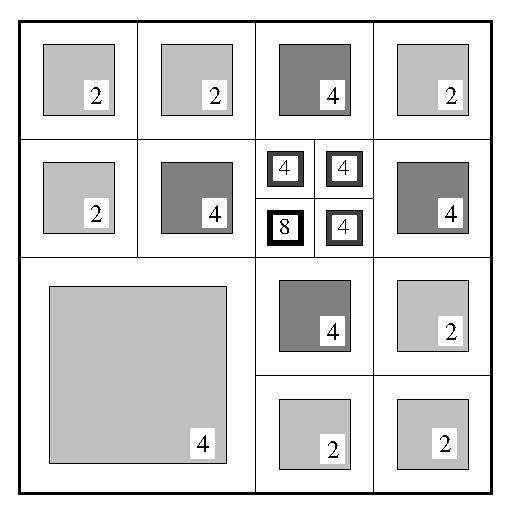
\includegraphics[width=1.8in]{amr2-9.eps} \ \
            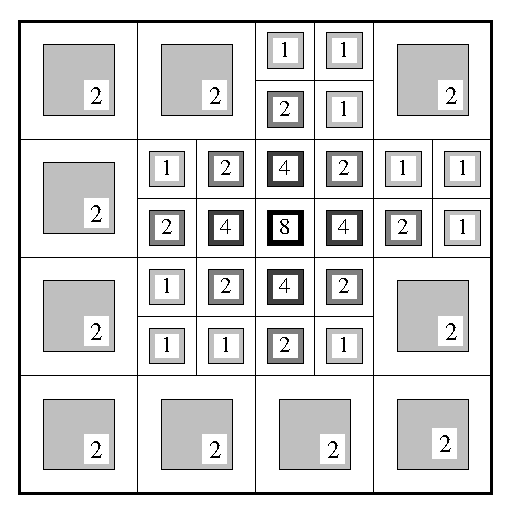
\includegraphics[width=1.8in]{amr2-11.eps}}

%-----------------------------------------------------------------------
\subsection{Use Cases}
%-----------------------------------------------------------------------
%-----------------------------------------------------------------------
\subsection{Parameters}
%-----------------------------------------------------------------------

%=======================================================================
\section{Array Component} \label{s:component-array}
%=======================================================================

Use chunked field storage \\
Field chunk size or range
The \code{Array} classes encapsulate Fortran-style arrays with
convenient operations and optional special features.  

Optional features include storing as a blocked array to improve cache
use, array padding to avoid cache thrashing on large power-of-two
arrays with low-associativity caches.  Arrays also may be parallelized
according to \code{Parallel} objects such as
\code{Parallel::Mpi} for MPI-parallel distributed arrays, or
\code{Parallel::Omp} for OpenMP-parallel threaded arrays (or both).

To manage the various optional features, Array classes use the
Decorator design pattern for dynamically adding special features at
run time:

 \centerline{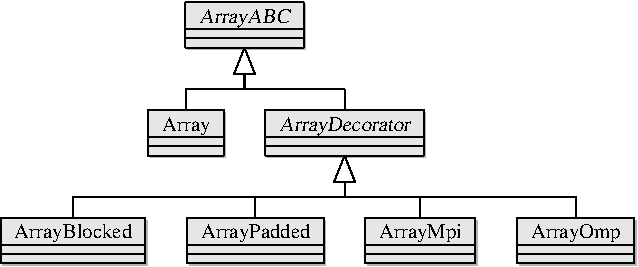
\includegraphics{uml/arrays.ps}}

\subsection{\code{Array}}

\centerline{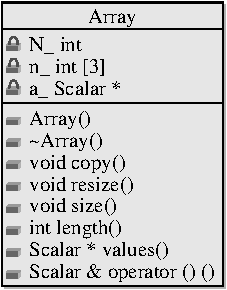
\includegraphics{uml/array.ps}}

\subsubsection{Array shape}

\subsubsection{Array blocking}

\subsubsection{Array padding}

\subsubsection{Array interleaving}


\subsection{Attributes}

\begin{tabbing}
xx\=xx\=xxxxxxxxxxxxxxxxxxxxxxxxxxxxxxxxxxx\= \kill
\> \todo \>  \textit{Length of array} \\
\>       \> \code{N\_: int }      \\ \\
\> \todo \>  \textit {Shape of array, right-padded with 1's} \\
\>       \> \code{n\_: int [3] }  \\ \\
\> \todo \>  \textit {Array values stored in column-major ordering}\\
\>       \> \code{a\_: Scalar * }
\end{tabbing}

\subsection{Operations}

\begin{tabbing}
xx\=xx\=xxxxxxxxxxxxxxxxxxxxxxxxxxxxxxxxxxx\= \kill
\> \todo \> \textit{Create a new uninitialized Array object} \\
\>       \> \code{Array()} \\ \\
\> \todo \> \textit{Create a new initialized Array object} \\
\>       \> \code{Array(int n0, int n1=1, int n2=1, int n3=1)} \\ \\
\> \todo \> \textit{Deallocate the array} \\
\>       \> \code{\~{\ }Array()}  \\ \\
\> \todo \> \textit{Copy an array into this one, deallocating any existing data} \\
\>       \> \code{void copy (const Array \&)}  \\ \\
\> \todo \> \textit{Resize the array, deallocating any existing data} \\
\>       \> \code{void resize (int n0, int n1=1, int n2=1, int n3=1)}   \\ \\
\> \todo \> \textit{Return the size of the array} \\
\>       \> \code{void size (int *n0, int *n1=0, int *n2=0, int *n3=0) const}  \\ \\
\> \todo \> \textit{Return the total length of the array} \\
\>       \> \code{int length () const}  \\ \\
\> \todo \> \textit{Return a pointer to the array values} \\
\>       \> \code{Scalar * values () const}  \\ \\
\> \todo \> \textit{Return the given array element} \\
\>       \> \code{Scalar \& operator () (int i0, int i1=0, int i2=0, int i3=0)}
\end{tabbing}



%=======================================================================
\section{Control parameters} \label{s:control}
%=======================================================================

Given Physics, Algorithms, and Data structures, specify the top-level
sequencing and properties of the simulation.  For example, ordering of
physics modules, whether to do hierarchical time-stepping, up to what
level, whether to sub-cycle some physics, etc. [Is this a useful
category?]  Also include things like floors and limits(?), and IO
dumps

Global simulation control.

Output types and parameters

\begin{itemize}
\item checkpoint (dump all)
\item output (specific fields)
\item movies (type and rate)
\item analysis (type of analysis, rate)
\item level of output (files for timestep, time, etc.)
\end{itemize}

%-----------------------------------------------------------------------
\subsection{Use Cases}
%-----------------------------------------------------------------------
%-----------------------------------------------------------------------
\subsection{Parameters}
%-----------------------------------------------------------------------


%=======================================================================
\section{Disk Component} \label{s:component-disk}
%=======================================================================

Output parameters.

%-----------------------------------------------------------------------
\subsection{Use Cases}
%-----------------------------------------------------------------------

\begin{verbatim}
output { 
   name = "data"
   format = hdf5
   type   = [data, input]
   fields = ["density", "velocity", "temperature"]
   file = ["data-%6s" cycle_number]
   cycle = 0:10:90
   cycle = 100:100:900
   cycle = 1000
}
\end{verbatim}

\begin{verbatim}
output { 
   name      = "restart"
   format    = hdf5
   type      = [data, input]
   fields    = all
   file      = ["restart-%6s" cycle_number]
   time_cpu  = 0.5 # CPU hours
   overwrite = true
   copies    = 2
}
\end{verbatim}

\begin{verbatim}
output { 
   name      = "movie"
   file      = ["movie-%6s" cycle_number]
   time      = :10:
   extract   = x == 12
}
\end{verbatim}


%-----------------------------------------------------------------------
\subsection{Parameters}
%-----------------------------------------------------------------------

Output types and parameters
 checkpoint (dump all)
 output (specific fields)
 movies (type and rate)
 analysis (type of analysis, rate)
 level of output (files for timestep, time, etc.)




%=======================================================================
\section{Error Component} \label{s:component-error}
%=======================================================================

Fault tolerance and adaptivity parameters

\begin{itemize}
\item fault tolerance methodology
\item adaptivity
\end{itemize}

%-----------------------------------------------------------------------
\subsection{Use Cases}
%-----------------------------------------------------------------------
%-----------------------------------------------------------------------
\subsection{Parameters}
%-----------------------------------------------------------------------

%=======================================================================
\section{Field Component} \label{s:component-field}
%=======================================================================

Scalar and vector fields for each material, such as
 density, energy, velocity, etc.  [Merge with Materials?]  Specify
 values, or input from files.

%-----------------------------------------------------------------------
\subsection{Use Cases}
%-----------------------------------------------------------------------
\begin{verbatim}
   field {
      name     = "density"
      name     = "rho"
      type     = scalar
      location = center
   }
   field {
      name     = "velocity"
      name     = "u"
      type     = vector
      location = center
   }
   field {
      name     = "temperature"
      name     = "T"
      type     = scalar
      location = center
   }
   field {
      name     = "B"
      type     = computed
      location = face
   }
\end{verbatim}

%-----------------------------------------------------------------------
\subsection{Parameters}
%-----------------------------------------------------------------------

%=======================================================================
\subsection{\code{Units} Component} \label{ss:component-units}
%=======================================================================

 Specify units and optional scalings for individual
 fields.  
 \note{Dynamic scaling, e.g.~to keep average of all fields near one.}

%-----------------------------------------------------------------------
\subsubsection{Use Cases}
%-----------------------------------------------------------------------
%-----------------------------------------------------------------------
\subsubsection{Parameters}
%-----------------------------------------------------------------------

%=======================================================================
\subsection{\code{Matter} Component} \label{ss:component-matter}
%=======================================================================

 Specify units and optional scalings for individual
 fields.  
 \note{Dynamic scaling, e.g.~to keep average of all fields near one.}

%-----------------------------------------------------------------------
\subsubsection{Use Cases}
%-----------------------------------------------------------------------

%-----------------------------------------------------------------------
\subsubsection{Parameters}
%-----------------------------------------------------------------------

\begin{verbatim}
   Matter {
      type = dark
   }
\end{verbatim}

\begin{verbatim}
   Matter {
      type  = gas_ideal
      gamma = 1.4
   }
\end{verbatim}


\subsection{ Field  Component}
Scalar fields on an Array or Mesh hierarchy

A Field represents a discretized scalar field. A Field is typically
discretized on an AMR hierarchy, but can be accessed at the Array or a
Block levels as well. In addition to the array of elements, a Field
includes an identifier for the field, the location of the field values
with respect to computational cells (cell centered, face-centered,
etc.), the index into the Block or Array of the field, optional
minimum or maximum allowed values, units, and user-defined tags.

Attributes:

\begin{tabular}{ll}
    \code{name}        & String defining the field's name, e.g. "density", "velocity-x", etc. \\
    \code{id} 	& Integer identifying the Field \\
    \code{array} &	Array containing Field values for the containing Patch \\
    \code{index} &	Index of the specific array in the 4D Array \\
    \code{position} &	cell position, defined as (0,0,0) <= (px,py,pz) <= (1,1,1). (.5,.5,.5)=cell centered \\
    \code{min} &	minimum allowed value for the Field \\
    \code{max} &	maximum allowed value for the Field \\
    \code{min\_action} &	what should be done if Field goes below min (e.g. 1: set to min, 2: warning, 4: error, g: retry with smaller timestep, etc.) \\
    \code{max\_action} &	what should be done if Field goes above max
\end{tabular}

A set of Fields defined on a Block, along with groups of Particles
associated with the block, are the main input to (and output from)
Methods. Methods have access to the Field's values, size, cell
position, units, tags, limits, etc.

Actual Field objects are stored in the Mesh Patch object. Patch objects
also contain associated Particle objects, and a Box object defining
the Patch's extents and position.  List of fields


Field supporting classes

Field operations
Field hierarchy
Structure
Descriptions
Field class
Attributes
Functions
Usage

Issues:

\begin{itemize}
\item What operations are the responsibility of Field versus Array,
  Task, Patch, etc.
\item see below: Field stores only global properties of field, not
  actual data
\item How to store global attributes (name, index, min, max, position,
  etc.) versus non-global (values)
\item Single global Field object for each field
\item Fields don't store actual Arrays, Patches do--Field only stores
  Array index.
\end{itemize}

%=======================================================================
\section{Memory Component} \label{s:component-memory}
%=======================================================================

Dynamic memory allocation.

%-----------------------------------------------------------------------
\subsection{Use Cases}
%-----------------------------------------------------------------------

%-----------------------------------------------------------------------
\subsection{Parameters}
%-----------------------------------------------------------------------




%=======================================================================
\section{Method Component} \label{s:component-method}
%=======================================================================

  Defines how to simulate the physics in the computational universe.
  A \code{Method} specifies the numerical method to use, which
  \code{Field}s are involved, and any associated method-specific
  parameters.  Sequencing and coupling of \code{Method}s is defined in
  \code{Problem} and implemented in \code{Control}.  Analysis and
  visualization are considered \code{Method}s as well.

\begin{itemize}
\item HD
\item MHD
\item RHD
\item cooling
\item gravity
\end{itemize}

Specify algorithms and their parameters.

HD dual-energy

HD steepening
HD flattening
HD diffusion

Timestepping


\begin{itemize}
\item PPM hydro (dual-energy, etc.)
\item gravity solver (FAC, smoother, levels, etc.)
\end{itemize}

%-----------------------------------------------------------------------
\subsection{Use Cases}
%-----------------------------------------------------------------------
%-----------------------------------------------------------------------
\subsection{Parameters}
%-----------------------------------------------------------------------

%=======================================================================
\subsection{Method:Hydro subcomponent}

%=======================================================================
\subsection{Method:Gravity subcomponent}

%=======================================================================
\subsection{Method:Cooling subcomponent}

%=======================================================================
\subsection{Method:Chemistry subcomponent}

%=======================================================================
\subsection{Method:MHD subcomponent}

%=======================================================================
\subsection{Method:RT subcomponent}

%=======================================================================
\subsection{Analysis subcomponent} \label{ss:component-analysis}
%=======================================================================

 Specify the algorithms and algorithm parameters to use for analysis
 and visualization.

%=======================================================================
\subsection{Visualization subcomponent} \label{ss:component-visualization}
%=======================================================================


%=======================================================================
\section{Monitor parameters} \label{s:monitor}
%=======================================================================

High-level monitoring of the run at a summary level, such as current
timestep, problem time, wall time, cpu time, etc.

%-----------------------------------------------------------------------
\subsection{Use Cases}
%-----------------------------------------------------------------------
\begin{verbatim}
   monitor {
     type   = html
     amount = verbose
   }
\end{verbatim}
%-----------------------------------------------------------------------
\subsection{Parameters}
%-----------------------------------------------------------------------


%=======================================================================
\section{Parallel Component} \label{s:component-parallel}
%=======================================================================

Hardware platform parallelism will be considered to be multilevel,
including nodes, processors, and cores.  Computational tasks will be
flexibly organized into hierarchical levels to aid mapping to multiple
hardware parallelization levels, including grid patches, grid patch
subblocks, and multiple simulations.  Task sizes in different levels
will allow flexibility to help optimize granularity for the different
given parallelization level components.

Flexible parallelism paradigms: map parallelism to tasks

Automatic code generation (or other) of parallel tasks to implement
parallelism and optimize performance

Specify parallelism type and parameters.  For example, non-blocking
MPI, MPI-2, hybrid MPI/UPC, performance-related parameters such as
buffer size, etc.

Specifiy parallelism and parameters

Specifiy method for controling parallelism

   parallelization method (MPI buffered/blocking, MPI2 Get)

\begin{itemize}
\item MPI (send/recv and type, one-sided and type, what level)
\item OpenMP (num threads, what level)
\item UPC (num threads, what level)
\item pthreads (num threads, what level)
\item cooperative parallelism
\item levels for each if multiple
\end{itemize}

%-----------------------------------------------------------------------
\subsection{Use Cases}
%-----------------------------------------------------------------------
%-----------------------------------------------------------------------
\subsection{Parameters}
%-----------------------------------------------------------------------

%=======================================================================
\subsection{MPI Send/Recv}

%=======================================================================
\subsection{MPI2 Get}

%=======================================================================
\subsection{OpenMP}

%=======================================================================
\subsection{Collaberative parallelism}

%=======================================================================
\subsection{Pipelining}



%=======================================================================
\section{Parameters Component} \label{s:component-parameters}
%=======================================================================

The \code{Parameters} component reads in a parameter file or files, and
provides the application access to parameter values.

        Stores user parameters, and provides functions to access
        parameter values.


%=======================================================================
\section{Particles Component} \label{s:component-particles}
%=======================================================================

Specifies data structures and data structure parameters related
to distributed particles.  

\begin{itemize}
\item min\_group\_size
\item max\_group\_size
\end{itemize}

%-----------------------------------------------------------------------
\subsection{Use Cases}
%-----------------------------------------------------------------------
%-----------------------------------------------------------------------
\subsection{Parameters}
%-----------------------------------------------------------------------


%=======================================================================
\section{Performance parameters} \label{s:performance}
%=======================================================================

Performance monitoring and optimization(?) parameters

%-----------------------------------------------------------------------
\subsection{Use Cases}
%-----------------------------------------------------------------------
%-----------------------------------------------------------------------
\subsection{Parameters}
%-----------------------------------------------------------------------


%=======================================================================
\section{Portal Component} \label{s:component-portal}
%=======================================================================
%-----------------------------------------------------------------------
\subsection{Use Cases}
%-----------------------------------------------------------------------
%-----------------------------------------------------------------------
\subsection{Parameters}
%-----------------------------------------------------------------------

%=======================================================================
\section{\code{Simulation} Component} \label{s:component-simulation}
%=======================================================================

Given \code{Physics}, \code{Methods}, and \code{Amr} or
\code{Particles} data structures, specifies and implements the
top-level sequencing and properties of the \code{Problem} (or
\code{Problems} in the case of an ensemble) to run.

\begin{itemize}
\item \code{Simulation}
\item \code{Ensemble}
\item \code{Control}
\item \code{Problem}
\item \code{Physics}
\item \code{Method}
\item \code{IO}
\end{itemize}

\subsection{Attributes.}

\subsection{Operations}

%=======================================================================
\subsection{\code{Ensemble} Component} \label{s:component-ensemble}
%=======================================================================

The \code{Ensemble} class is used to define a ensemble of simulations.  

\subsection{Attributes.}

\subsection{Operations}


%=======================================================================
\subsection{Control Component} \label{ss:component-control}
%=======================================================================


Global simulation control.

Output types and parameters

\begin{itemize}
\item checkpoint (dump all)
\item output (specific fields)
\item movies (type and rate)
\item analysis (type of analysis, rate)
\item level of output (files for timestep, time, etc.)
\end{itemize}

%-----------------------------------------------------------------------
\subsection{Use Cases}
%-----------------------------------------------------------------------
%-----------------------------------------------------------------------
\subsection{Parameters}
%-----------------------------------------------------------------------

Problem parameters specify the setup of the physical problem,
including initial conditions of relevant data fields and boundary
conditions.

  dimensionality
  domain extents
  initial conditions (materials, subregions, input)
 boundary conditions (periodic, in-/out-flow, specified, dynamic)

Problem parameters include initial conditions and boundary conditions.

Different types of boundary conditions are supported, including
periodic, in- and out-flow, specified, and dynamic.  Different
boundary conditions can be specified for the entire domain, on
separate faces, on subregions of faces, or on specific zones.
Different boundary conditions can be specified for different fields.
%-----------------------------------------------------------------------
\subsection{Use Cases}
%-----------------------------------------------------------------------

\begin{verbatim}
   problem {
      boundary {
         x:lower = reflecting
         x:upper = { type = reflecting }
         y       = { type = periodic }
         z       = { type = inflow,  value = 1.0 }
         z       = { outflow, 1.0 }
      }
   }
\end{verbatim}

\begin{verbatim}
   XM = boundary { x = domain:lower[0] }
   XP = boundary { x = domain:upper[0] }
   YM = boundary { y = domain:lower[1] }
   YP = boundary { y = domain:upper[1] }
   ZM = boundary { z = domain:lower[2] }
   ZP = boundary { z = domain:upper[2] }
   field {
      name = "density"
      value(XM) = 0
      value(XP) = 0
      value(YM) = value (YP)
      value(ZM) = +t
      value(ZM) = -t
   }
\end{verbatim}

%=======================================================================
\subsection{Domain} \label{ss:component-domain}
%=======================================================================

The \code{domain} function is used to specify properties of the
domain.  Domains are boxes aligned with the axes of the computational
coordinate system, and are uniquely determined by the spacial
dimension, and the lowest and highest points in the domain.

%-----------------------------------------------------------------------
\subsubsection{Use Cases}
%-----------------------------------------------------------------------

\begin{verbatim}
   domain { 
      dimension = 3
      lower     = <-3e9,-3e9,-3e9>
      upper     = <3e9,3e9,3e9>
   }
\end{verbatim}

\begin{verbatim}
   domain { 3, <-3e9,-3e9,-3e9>, <3e9,3e9,3e9> }  // Implicit ordering
\end{verbatim}

\begin{verbatim}
   domain { 
      dimension = 3
      upper     = 3e9        // expand scalar to vector
      lower     = -upper     // parameters can be accessed as values
   }
\end{verbatim}

Include errors.

%-----------------------------------------------------------------------
\subsubsection{Parameters}
%-----------------------------------------------------------------------

 \todo\ \textit{Decide: allow defaults?  allow optional parameters?  Special
 \code{OPT\_} prefix for optional parameters?  Write out explicit copy
 of input file?}

The \code{domain} function has three parameters

\begin{tabular}{lll} \\
Name & Type & Restrictions \\ \hline
\code{dimension} & Scalar & $1-3$ \\
\code{lower}     & Vector & length = \code{dimension} \\
\code{upper}     & Vector & length = \code{dimension}, \code{upper} $>$ \code{lower}
\end{tabular}

Lower and upper points are given in units given by \code{units},
described in \S\ref{ss:params-units}.

%-----------------------------------------------------------------------
\subsubsection{Restrictions}
%-----------------------------------------------------------------------

\begin{enumerate}
\item The dimension must be 1, 2, or 3.
\item The number of coordinates in both lower and upper points must equal the dimension.
\item Each coordinate of the lower point must be strictly greater than the corresponding coordinate of the upper point.
\end{enumerate}


%-----------------------------------------------------------------------
\subsubsection{Parameters}
%-----------------------------------------------------------------------

%-----------------------------------------------------------------------
\subsection{\code{Boundary}} \label{ss:component-boundary}
%-----------------------------------------------------------------------

The \code{Boundary} class is used to define the boundary conditions on
the domain.

%-----------------------------------------------------------------------
\subsection{\code{Initial}} \label{s:component-initial}
%-----------------------------------------------------------------------

The \code{Initial} class is used to define the initial conditions for
a problem.




%=======================================================================
\section{Task Component} \label{s:component-task}
%=======================================================================



% %=======================================================================
\section{Control parameters} \label{s:control}
%=======================================================================

Given Physics, Algorithms, and Data structures, specify the top-level
sequencing and properties of the simulation.  For example, ordering of
physics modules, whether to do hierarchical time-stepping, up to what
level, whether to sub-cycle some physics, etc. [Is this a useful
category?]  Also include things like floors and limits(?), and IO
dumps

Global simulation control.

Output types and parameters

\begin{itemize}
\item checkpoint (dump all)
\item output (specific fields)
\item movies (type and rate)
\item analysis (type of analysis, rate)
\item level of output (files for timestep, time, etc.)
\end{itemize}

%-----------------------------------------------------------------------
\subsection{Use Cases}
%-----------------------------------------------------------------------
%-----------------------------------------------------------------------
\subsection{Parameters}
%-----------------------------------------------------------------------


% %=======================================================================
\section{Parameters Component} \label{s:component-parameters}
%=======================================================================

The \code{Parameters} component reads in a parameter file or files, and
provides the application access to parameter values.

        Stores user parameters, and provides functions to access
        parameter values.


% %=======================================================================
\section{Units parameters} \label{s:units}
%=======================================================================

 Specify units and optional scalings for individual
 fields.  [Merge units with Control?] [Merge scaling with Fields?] 
 [Dynamic scaling, e.g.~to keep average of all fields near one.]

%-----------------------------------------------------------------------
\subsection{Use Cases}
%-----------------------------------------------------------------------
%-----------------------------------------------------------------------
\subsection{Parameters}
%-----------------------------------------------------------------------

% %=======================================================================
\section{Domain Component} \label{s:component-domain}
%=======================================================================

The \code{domain} function is used to specify properties of the
domain.  Domains are boxes aligned with the axes of the computational
coordinate system, and are uniquely determined by the spacial
dimension, and the lowest and highest points in the domain.

%-----------------------------------------------------------------------
\subsection{Use Cases}
%-----------------------------------------------------------------------

\begin{verbatim}
   domain { 
      dimension = 3
      lower     = <-3e9,-3e9,-3e9>
      upper     = <3e9,3e9,3e9>
   }
\end{verbatim}

\begin{verbatim}
   domain { 3, <-3e9,-3e9,-3e9>, <3e9,3e9,3e9> }  // Implicit ordering
\end{verbatim}

\begin{verbatim}
   domain { 
      dimension = 3
      upper     = 3e9        // expand scalar to vector
      lower     = -upper     // parameters can be accessed as values
   }
\end{verbatim}

Include errors.

%-----------------------------------------------------------------------
\subsection{Parameters}
%-----------------------------------------------------------------------

 \todo\ \textit{Decide: allow defaults?  allow optional parameters?  Special
 \code{OPT\_} prefix for optional parameters?  Write out explicit copy
 of input file?}

The \code{domain} function has three parameters

\begin{tabular}{lll} \\
Name & Type & Restrictions \\ \hline
\code{dimension} & Scalar & $1-3$ \\
\code{lower}     & Vector & length = \code{dimension} \\
\code{upper}     & Vector & length = \code{dimension}, \code{upper} $>$ \code{lower}
\end{tabular}

Lower and upper points are given in units given by \code{units},
described in \S\ref{s:units}.

%-----------------------------------------------------------------------
\subsection{Restrictions}
%-----------------------------------------------------------------------

\begin{enumerate}
\item The dimension must be 1, 2, or 3.
\item The number of coordinates in both lower and upper points must equal the dimension.
\item Each coordinate of the lower point must be strictly greater than the corresponding coordinate of the upper point.
\end{enumerate}



% \input{      component-boundary}
% \input{      component-initial}
% %=======================================================================
\section{Matter Component} \label{s:component-matter}
%=======================================================================

 Matter defines properties of matter, such as the matter type (baryonic
 or dark matter), and gas constants.

%-----------------------------------------------------------------------
\subsection{Use Cases}
%-----------------------------------------------------------------------

\begin{verbatim}
   Matter {
      type = dark
   }
\end{verbatim}

\begin{verbatim}
   Matter {
      type  = gas_ideal
      gamma = 1.4
      region { (x < 0) || (x > 1) }
   }
\end{verbatim}
%-----------------------------------------------------------------------
\subsection{Parameters}
%-----------------------------------------------------------------------

% \input{   component-analysis}
% %=======================================================================
\section{Data Component} \label{s:component-data}
%=======================================================================

Specify low-level datastructures (fields and particles) and their
parameters.

Use chunked field storage \\
Field chunk size or range


%=======================================================================
\subsection{Arrays}

%=======================================================================
\subsection{Fields}

%=======================================================================
\subsection{Particles}

%=======================================================================
\subsection{Structured Adaptive Mesh Hierarchies}

%=======================================================================
\subsection{Octree}


% 
%=======================================================================
\section{Performance parameters} \label{s:performance}
%=======================================================================

Performance monitoring and optimization(?) parameters

%-----------------------------------------------------------------------
\subsection{Use Cases}
%-----------------------------------------------------------------------
%-----------------------------------------------------------------------
\subsection{Parameters}
%-----------------------------------------------------------------------

